\begin{figure}[!htbp]
\begin{center}
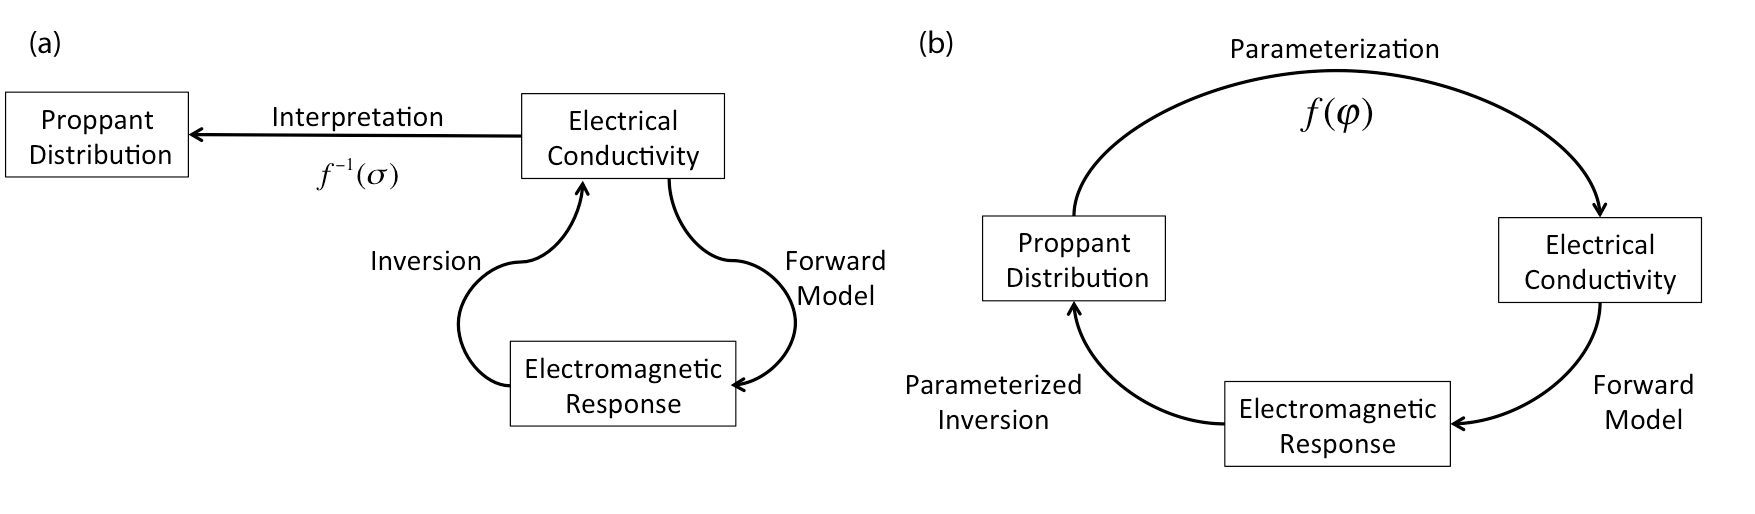
\includegraphics[width=0.9\textwidth]{figures/simpeg/heagy2014.png}
\end{center}
\caption{
(a) Traditional approach to inversion, where the model space, electrical conductivity, is mapped to data space, the electromagnetic response, through a forward model. The inversion then provides a method by which we estimate a model that is consistent with the observed data. The recovered conductivity model is then used to infer information about the reservoir properties of interest, in this case, the distribution of proppant. (b) Parametrized inversion, where we parametrize the model space, electrical conductivity, in terms of the property of interest, the distribution of proppant. By defining such a parametrization, the inversion can provide a means of estimating the properties of interest directly from the data.
}
\label{fig:simpeg-heagy2014}
\end{figure}
